\documentclass[english,floatsintext,man]{apa6}

\usepackage{amssymb,amsmath}
\usepackage{ifxetex,ifluatex}
\usepackage{fixltx2e} % provides \textsubscript
\ifnum 0\ifxetex 1\fi\ifluatex 1\fi=0 % if pdftex
  \usepackage[T1]{fontenc}
  \usepackage[utf8]{inputenc}
\else % if luatex or xelatex
  \ifxetex
    \usepackage{mathspec}
    \usepackage{xltxtra,xunicode}
  \else
    \usepackage{fontspec}
  \fi
  \defaultfontfeatures{Mapping=tex-text,Scale=MatchLowercase}
  \newcommand{\euro}{€}
\fi
% use upquote if available, for straight quotes in verbatim environments
\IfFileExists{upquote.sty}{\usepackage{upquote}}{}
% use microtype if available
\IfFileExists{microtype.sty}{\usepackage{microtype}}{}

% Table formatting
\usepackage{longtable,booktabs}
\usepackage[counterclockwise]{rotating}   % Landscape page setup for large tables
\usepackage{multirow}		% Table styling
\usepackage{tabularx}		% Control Column width
\usepackage[flushleft]{threeparttable}	% Allows for three part tables with a specified notes section
\usepackage{threeparttablex}            % Lets threeparttable work with longtable
\usepackage{longtable}              % Allows tables to break across pages

  \usepackage{graphicx}
  \makeatletter
  \def\maxwidth{\ifdim\Gin@nat@width>\linewidth\linewidth\else\Gin@nat@width\fi}
  \def\maxheight{\ifdim\Gin@nat@height>\textheight\textheight\else\Gin@nat@height\fi}
  \makeatother
  % Scale images if necessary, so that they will not overflow the page
  % margins by default, and it is still possible to overwrite the defaults
  % using explicit options in \includegraphics[width, height, ...]{}
  \setkeys{Gin}{width=\maxwidth,height=\maxheight,keepaspectratio}
\ifxetex
  \usepackage[setpagesize=false, % page size defined by xetex
              unicode=false, % unicode breaks when used with xetex
              xetex]{hyperref}
\else
  \usepackage[unicode=true]{hyperref}
\fi
\hypersetup{breaklinks=true,
            pdfauthor={},
            pdftitle={A Quantitative Synthesis of Early Language Acquisition Using Meta-Analysis},
            colorlinks=true,
            citecolor=blue,
            urlcolor=blue,
            linkcolor=black,
            pdfborder={0 0 0}}
\urlstyle{same}  % don't use monospace font for urls

\setlength{\parindent}{0pt}
%\setlength{\parskip}{0pt plus 0pt minus 0pt}

\setlength{\emergencystretch}{3em}  % prevent overfull lines

\setcounter{secnumdepth}{0}
\ifxetex
  \usepackage{polyglossia}
  \setmainlanguage{}
\else
  \usepackage[english]{babel}
\fi

% Manuscript styling
\captionsetup{font=singlespacing,justification=justified}
\usepackage{csquotes}



\usepackage{tikz} % Variable definition to generate author note

% fix for \tightlist problem in pandoc 1.14
\providecommand{\tightlist}{%
  \setlength{\itemsep}{0pt}\setlength{\parskip}{0pt}}

% Essential manuscript parts
  \title{A Quantitative Synthesis of Early Language Acquisition Using
Meta-Analysis}

  \shorttitle{A Quantitative Synthesis}


  \author{
          Molly Lewis\textsuperscript{1},
          Mika Braginsky\textsuperscript{1},
          Sho Tsuji\textsuperscript{2},
          Christina Bergmann\textsuperscript{2},
          Page Piccinini\textsuperscript{2},
          Alejandrina Cristia\textsuperscript{2},
          Michael C. Frank\textsuperscript{1}  }

  \def\affdep{{"", "", "", "", "", "", ""}}%
  \def\affcity{{"", "", "", "", "", "", ""}}%

  \affiliation{
    \vspace{0.5cm}
          \textsuperscript{1} Department Psychology, Stanford University\\
          \textsuperscript{2} Laboratoire de Sciences Cognitives et Psycholinguistique, ENS  }


%   \def\affinst{{"init", "Department Psychology, Stanford University", "Laboratoire de Sciences Cognitives et Psycholinguistique, ENS"}}%
%   \def\affstate{{"init", "", ""}}%
%   \def\affcntry{{"init", "", ""}}%

  \note{
    \vspace{1cm}
    Author note

    \raggedright
    \setlength{\parindent}{0.4in}

    \newcounter{author}

%     %     %       %       \setcounter{author}{0}
%         %           \addtocounter{author}{1}
%         %         \expandafter\edef\csname authorid\endcsname{\theauthor}
%         Molly Lewis, \pgfmathparse{\affdep[\authorid]} \pgfmathresult, \pgfmathparse{\affinst[\authorid]} \pgfmathresult, \pgfmathparse{\affcity[\authorid]} \pgfmathresult, \pgfmathparse{\affstate[\authorid]} \pgfmathresult, \pgfmathparse{\affcntry[\authorid]} \pgfmathresult
%       %     ;
%     %       %       \setcounter{author}{0}
%         %           \addtocounter{author}{1}
%         %         \expandafter\edef\csname authorid\endcsname{\theauthor}
%         Mika Braginsky, \pgfmathparse{\affdep[\authorid]} \pgfmathresult, \pgfmathparse{\affinst[\authorid]} \pgfmathresult, \pgfmathparse{\affcity[\authorid]} \pgfmathresult, \pgfmathparse{\affstate[\authorid]} \pgfmathresult, \pgfmathparse{\affcntry[\authorid]} \pgfmathresult
%       %     ;
%     %       %       \setcounter{author}{0}
%         %           \addtocounter{author}{2}
%         %         \expandafter\edef\csname authorid\endcsname{\theauthor}
%         Sho Tsuji, \pgfmathparse{\affdep[\authorid]} \pgfmathresult, \pgfmathparse{\affinst[\authorid]} \pgfmathresult, \pgfmathparse{\affcity[\authorid]} \pgfmathresult, \pgfmathparse{\affstate[\authorid]} \pgfmathresult, \pgfmathparse{\affcntry[\authorid]} \pgfmathresult
%       %     ;
%     %       %       \setcounter{author}{0}
%         %           \addtocounter{author}{2}
%         %         \expandafter\edef\csname authorid\endcsname{\theauthor}
%         Christina Bergmann, \pgfmathparse{\affdep[\authorid]} \pgfmathresult, \pgfmathparse{\affinst[\authorid]} \pgfmathresult, \pgfmathparse{\affcity[\authorid]} \pgfmathresult, \pgfmathparse{\affstate[\authorid]} \pgfmathresult, \pgfmathparse{\affcntry[\authorid]} \pgfmathresult
%       %     ;
%     %       %       \setcounter{author}{0}
%         %           \addtocounter{author}{2}
%         %         \expandafter\edef\csname authorid\endcsname{\theauthor}
%         Page Piccinini, \pgfmathparse{\affdep[\authorid]} \pgfmathresult, \pgfmathparse{\affinst[\authorid]} \pgfmathresult, \pgfmathparse{\affcity[\authorid]} \pgfmathresult, \pgfmathparse{\affstate[\authorid]} \pgfmathresult, \pgfmathparse{\affcntry[\authorid]} \pgfmathresult
%       %     ;
%     %       %       \setcounter{author}{0}
%         %           \addtocounter{author}{2}
%         %         \expandafter\edef\csname authorid\endcsname{\theauthor}
%         Alejandrina Cristia, \pgfmathparse{\affdep[\authorid]} \pgfmathresult, \pgfmathparse{\affinst[\authorid]} \pgfmathresult, \pgfmathparse{\affcity[\authorid]} \pgfmathresult, \pgfmathparse{\affstate[\authorid]} \pgfmathresult, \pgfmathparse{\affcntry[\authorid]} \pgfmathresult
%       %     ;
%     %       %       \setcounter{author}{0}
%         %           \addtocounter{author}{1}
%         %         \expandafter\edef\csname authorid\endcsname{\theauthor}
%         Michael C. Frank, \pgfmathparse{\affdep[\authorid]} \pgfmathresult, \pgfmathparse{\affinst[\authorid]} \pgfmathresult, \pgfmathparse{\affcity[\authorid]} \pgfmathresult, \pgfmathparse{\affstate[\authorid]} \pgfmathresult, \pgfmathparse{\affcntry[\authorid]} \pgfmathresult
%       %     .
%     
    Correspondence concerning this article should be addressed to Molly
    Lewis, Psychology Department, Stanford University. 450 Serra Mall,
    Stanford, CA 94305. E-mail:
    \href{mailto:mll@stanford.edu}{\nolinkurl{mll@stanford.edu}}.

                                                                                    }

  \abstract{replicability, etc.}
  \keywords{developmental psychology,
language acquisition, quantitative theories, meta-analysis \\

    \indent Word count: XXXX
  }

  \usepackage{setspace}
  \usepackage{float}
  \usepackage{graphicx}
  \AtBeginEnvironment{tabular}{\singlespacing}
  \usepackage{pbox}

\begin{document}

\maketitle



\section{Introduction}\label{introduction}

To learn to speak a language, a child must acquire a wide range of
knowledge and skills: the sounds of the language, the word forms, and
the mappings of words to meanings, to name only a few. How does this
process unfold? Our goal as psychologists is to build a theory that can
explain and predict this process. But, acquiring a language requires not
just learning these skills in isolation; it requires the integration of
a range of skills across the language hierarchy. Consider, for example,
a child learning the word \enquote{dog:} If the child is unable to
segment the word from natural speech, learning the meaning of this word
is impossible. In building a theory of this system, a pragmatic research
strategy has been to study these skills primarily in isolation,
describing the developmental trajectory of individual phenomena in
separate research programs. However, if it is indeed the case that
linguistic skills are interdependent, ultimately we may not be able to
understand one skill without a more precise understanding of the broader
system.

The theory building effort is further complicated by the fact that we
must do so on the basis of limited, noisy experimental findings. These
limited findings mean that the raw material of our theories are often
contradictory, with one study finding an effect, but another failing to
do so. These contradictions leave the theorist with uncertainty about
which experimental findings should constrain the theory. What is needed
then is a method for determining the degree to which a particular
findings provides evidence for a theory.

We suggest a solution to both of these challenges---building integrative
theories and evaluating evidential strength---is to reframe experimental
findings in terms of quantitative, rather than qualitative,
descriptions. Quantitative descriptions allow for the use of
quantitative methods for aggregating experimental findings in order to
evaluate evidential strength. In addition, describing experimental
findings as quantitative estimates provides a common language for
comparing across phenomenon, and a way to make more precise predictions.
In this paper, we consider the domain of language acquisition and
demonstrate how a set of quantitative tools---meta-analysis---can
support these two theory-building goals.

Meta-analysis is a quantitative method for aggregating across
experimental findings. The fundamental unit of meta-analysis is the
\emph{effect size}: a scale-free, quantitative measure of
\enquote{success} in a phenomenon. Importantly, an effect size provides
an estimate of the \emph{size} of an effect, as well as a measure of
uncertainty around this point estimate. With such a quantitative measure
of success, we can apply the same reasoning we use to aggregate noisy
measurements over participants in a single study: By assuming each
\emph{study}, rather than participant, is sampled from a population, we
can appeal to the classical statistical framework to combine estimates
of the effect size for a given phenomenon.

Meta-analytic methods support theory building in several ways. First,
they provide a way to evaluate which effects in a literature are most
likely to be observed consistently, and thus should constrain the
theory. This issue is particularly important in light of recent
high-profile evidence that an effect observed in one study may not
replicate in another (``replication crisis,'' Ioannidis, 2005; Open
Science Collaboration, 2012, 2015). Failed replications are difficult to
interpret, however, because they may result from a wide variety of
causes, including an initial false positive, a subsequent false
negative, or differences between initial and replication studies, and
making causal attributions in a situation with two conflicting studies
is often difficult (Anderson et al., 2016; Gilbert, King, Pettigrew, \&
Wilson, 2016). By aggregating evidence across studies and assuming that
there is some variability in true effect size from study to study. In
this way, meta-analytic methods can provide more veridical description
of the empirical landscape, which in turn leads to better
theory-building.

Second, meta-analysis supports theory building by providing higher
fidelity descriptions of phenomena. Given an effect size estimate,
meta-analytic methods provide a method for quantifying the amount
variability around this point estimate. Furthermore, the quantitative
framework allows researchers to detect potential moderators in effect
size. This ability is particularly important for developmental phenomena
because building a theory requires a precise description of changes in
effect size across development. Individual papers typically describe an
effect size for 1-2 age groups, but the ultimate goal is to detect a
moderator---age---in this effect. Given that moderator always require
more power to detect (Button et al., 2013), it may be quite difficult to
detect developmental trends in effect sizes from individual papers. By
aggregating across papers through meta-analytic methods, however, we may
be able to detect these changes, leading to a more precise description
of the empirical phenomena.

In addition to providing a quantitative measure of success, effect size
estimates also provide a common language for comparing \emph{across}
phenomena. In the current work, this common language allows us to
meaningfully consider the relationship between different phenomena in
the language acquisition domain (\enquote{meta-meta-analysis}). Through
cross-phenomena comparisons, we can understand not only the trajectory
of a particular phenomenon, like word learning for example, but also how
this phenomenon might relate to other skills, such as sound learning,
gaze following, and many others.

Finally, in addition to these theoretical motivations, there are
practical reasons for conducting a quantitative synthesis. When planning
an experiment, an estimate of the size of an effect on the basis of
prior literature can inform the sample size needed to achieve a desired
level of power. Meta-analytic estimates of effect sizes can also aid in
design choices: If a certain paradigm or measure tends to yield overall
larger effect sizes than another, the strategic researcher might select
this paradigm in order to maximize the power achieved with a given
sample size.

Language acquisition may be a particularly informative application for
meta-analytic tools, although these tools are broadly applicable to
psychological literatures. One reason is that language acquisition may
be uniquely vulnerable to false findings because running children is
expensive, and thus sample sizes are small and studies are underpowered
(Ioannidis, 2005). In addition, the high cost and practical difficulties
associated with collecting large developmental datasets means that
replications are relatively rare in the field. Finally, there has been
attention to research practices in developmental psychology broadly,
suggesting evidence of experimenter bias (Peterson, 2016).

We take as our ultimate goal a broad theory of language acquisition that
can explain and predict the range of linguistic skills a child acquires.
Toward this end, we developed a dataset of effect sizes in the language
acquisition literature across 12 core phenomena
(\href{http://metalab.stanford.edu}{Metalab;
http://metalab.stanford.edu/}). We demonstrate how meta-analysis
supports building this theory in two ways. We first use meta-analytic
techniques to evaluate the evidential value of the empirical landscape
in language acquisition research. We find broadly that this literature
has strong evidential value, and thus that the effects reported in the
literature should constrain our theorizing of language acquisition. We
then turn toward the task of synthesizing these findings across
phenomena and offer a preliminary theoretical synthesis of the field.

\section{Method}\label{method}

We analyzed 12 different phenomena in language acquisition. These
particular phenomena were selected opportunistically, either because of
high prevalence in the literature or because a published meta-analysis
already existed. The phenomena cover development at many different
levels of the language hierarchy, from the acquisition of prosody and
phonemic contrasts, to gaze following in communicative interaction. This
wide range of phenomena allowed us to compare the course of development
across different domains, as well as to explore questions about the
interactive nature of language acquisition (Table 1).

To obtain estimates of effect size, we coded papers reporting
experimental data (see SI for details). Within each paper, we calculated
a separate effect size estimate for each experiment and age group (we
refer to this as a \enquote{condition}). In total, our sample includes
estimates from 269 papers, 981 different conditions and 12,029
participants. {[}RELIABILITY CODING?{]} The process for selecting papers
from the literature differed by domain, with some individual
meta-analyses using more systematic approaches than others (see SI).
\renewcommand{\arraystretch}{1.5}

\begin{table}[h!]
        \footnotesize
        \begin{tabular}{lp{4cm} p{5cm}r}
            \toprule
            \textbf{Level} & \textbf{Phenomenon}                                                               & \textbf{Description}                                                                                 & \textbf{N papers (conditions)}                                                                                                                                               \\
                        \midrule

            Prosody        & IDS  preference  \newline  {\scriptsize (Dunst, Gorman, \& Hamby, 2012)}          & {\scriptsize  Looking times as a function of whether infant-directed vs. adult-directed speech is presented as stimulation.}      & 16 (50)     \\
            Sounds         & Phonotactic learning  \newline {\scriptsize (Cristia, in prep.)}                   & {\scriptsize Infants' ability to learn phonotactic generalizations from a short exposure.  }                  & 15 (47)                               \\
            ~              & Vowel discrimination (native) \newline {\scriptsize (Tsuji \& Cristia, 2014)}     & {\scriptsize Discrimination of native-language vowels, including results from a variety of methods.  }         & 40 (167)             \\ 
            ~              & Vowel discrimination (non-native) \newline {\scriptsize (Tsuji \& Cristia, 2014)} & {\scriptsize Discrimination of non-native vowels, including results from a variety of methods.  }     & 21 (72)     \\
               & Statistical sound learning  \newline {\scriptsize (Cristia, in prep.)}             & {\scriptsize Infants' ability to learn sound categories from their acoustic distribution.   }  & 11 (40) \\ 
            & Word segmentation \newline {\scriptsize  (Bergmann \& Cristia, 2015) }            & {\scriptsize Recognition of familiarized words from running, natural speech using behavioral methods.  }                     & 68 (296)                                     \\
            Words     &   Mutual exclusivity \newline {\scriptsize (Lewis \& Frank, in prep.)} &{\scriptsize  Mapping of novel words reflecting children's inference that novel words tend to refer to novel objects.}
            & 20 (60)             \\
            ~ &   Sound Symbolism \newline {\scriptsize (Lammertink et al., in prep.)} &{\scriptsize  Non-arbitrary relationship between form and meaning ("bouba-kiki effect").}
            & 10 (42)             \\
            ~              & Concept-label advantage   \newline {\scriptsize (Lewis \& Long, unpublished)}     & {\scriptsize Infants' categorization judgments in the presence and absence of labels.    } & 16 (100) \\
            ~              & Online word recognition \newline {\scriptsize (Frank, Lewis, \& MacDonald, 2016)} & {\scriptsize Online word recognition of familiar words using two-alternative forced choice preferential looking.   }              & 12 (32)                         \\
            Communication  & Gaze following  \newline {\scriptsize  (Frank, Lewis, \& MacDonald, 2016)}        & {\scriptsize Gaze following using standard multi-alternative forced-choice paradigms.   }                       & 15 (45)                                           \\
            ~              & Pointing and vocabulary  \newline {\scriptsize (Colonnesi et al., 2010)}          & {\scriptsize Longitudinal correlations between declarative pointing and later vocabulary.  }               & 25 (30)                         \\ 
            \bottomrule
        \end{tabular}
        \caption{Overview of meta-analyses in dataset.}
    \end{table}

\section{Replicability of the field}\label{replicability-of-the-field}

To assess the replicability of language acquisition phenomena, we
conducted several diagnostic analyses: Meta-analytic estimates of effect
size, fail-safe-N (Orwin, 1983), funnel plots, and p-curve (Simonsohn,
Nelson, \& Simmons, 2014b, 2014a; Simonsohn, Simmons, \& Nelson, 2015).
These analytical approaches each have limitations, but taken together,
they provide converging evidence about whether a true effect is likely
to exist, and the extent to which publication bias and other
questionable research practices are present in the literature. Overall,
we find most phenomena in the language acquisition literature have
evidential value, and should therefore provide the basis for theoretical
development. We also find evidence for some bias, as well as evidence
that two phenomena---phonotactic learning and statistical sound
learning---likely describe null or near-null effects.

\subsection{Meta-Analytic Effect Size}\label{meta-analytic-effect-size}

To estimate the overall effect size of a literature, effect sizes are
pooled across papers to obtain a single meta-analytic estimate. This
meta-analytic effect-size can be thought of as the \enquote{best
estimate} of the effect size for a phenomenon given all the available
data in the literature.

Table 2, column 2 presents meta-analytic effect size estimates for each
of our phenomena. We find evidence for a non-zero effect size in 11 out
of 12 of the phenomena in our dataset, suggesting these literatures
provide evidential value. In the case of phonotactic learning, however,
we find that the meta-analytic effect size estimate does not differ from
zero, suggesting that this literature does not describe a robust effect.

We next turn to methods of assessing evidential value that describe the
\emph{degree} to which a literature has evidential value, and thus the
degree to which it should constrain our theory building. In the
following three analyses---fail-safe-N, funnel plots, and p-curves---we
attempt to quantify the evidential value of these literatures.

\subsection{Fail-safe-N}\label{fail-safe-n}

One approach for quantifying the reliability literature is to ask, How
many missing studies with null effects would have to exist in the
\enquote{file drawer} in order for the overall effect size to be zero?
This is called the \enquote{fail-safe} number of studies (Orwin, 1983).
This number provides an estimate of the size and variance of an effect
using the intuitive unit of studies. To estimate this number, we
estimated the overall effect size for each phenomenon (Table 2, column
2), and then used this to estimate the fail-safe-N (Table 2, column 3).

Because of the large number of positive studies in many of the
meta-analyses we assessed, this analysis suggests a very large number of
studies would have to be \enquote{missing} in each literature (\(M\) =
3634) in order for the overall effect sizes to be 0. Thus, while it is
possible that some reporting bias is present in the literature, the
large fail-safe-N suggests that the literature nonetheless likely
describes a real effect.

This analysis provides a quantitative estimate of the size of an effect
in an intuitive unit, but it does not assess analytical or publication
bias (CITE). Importantly, if experimenters are exercising analytical
flexibility through practices like p-hacking, then the number and
magnitude of observed true effects in the literature may be greatly
inflated. In the next analysis, we assess the presence of bias through
funnel plots.

\subsection{Funnel Plots}\label{funnel-plots}

Funnel plots provide a visual method for evaluating whether variability
in effect sizes is due only to differences in sample size. A funnel plot
shows effect sizes versus a metric of sample size, standard error. If
there is no bias in a literature, we should expect studies to be
randomly sampled around the mean, with more variability for less precise
studies.

Figure 1 presents funnel plots for each of our 12 meta-analyses. These
plots show evidence of asymmetry (bias) for several of our phenomenon
(Table 2, column 4). However, an important limitation of this method is
that it is difficult to determine the source of this bias. One
possibility is that this bias reflects true heterogeneity in phenomena
(e.g.~different
ages)\footnote{The role of moderators such as age can be interactively explored on the website, [Metalab; http://metalab.stanford.edu/](http://metalab.stanford.edu).}.
P-curve analyses provide one method for addressing this issue, which we
turn to next.

\begin{figure}[htbp]
\centering
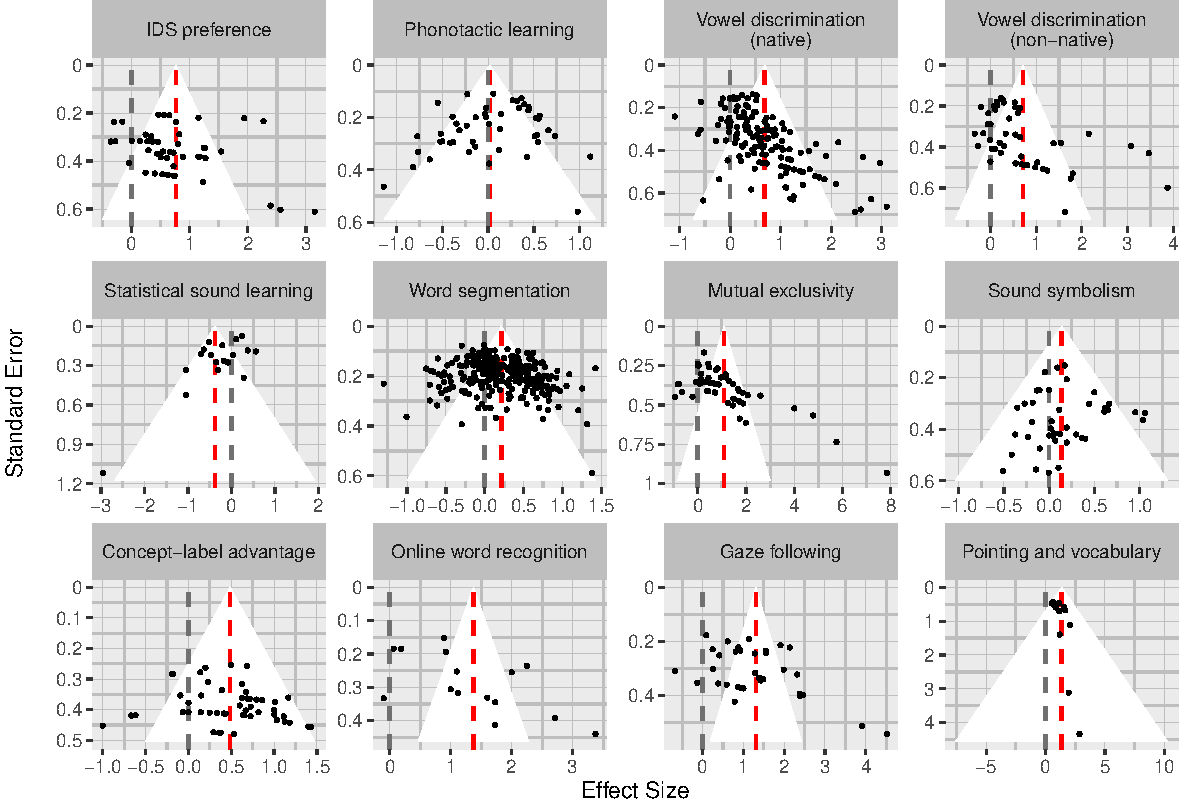
\includegraphics{metalab_synthesis_files/figure-latex/unnamed-chunk-2-1.pdf}
\caption{Funnel plots for each meta-analysis. Each effect size estimate
is represented by a point, and the mean effect size is shown as a red
dashed line. The funnel corresponds to a 95\% CI around this mean. In
the absence of true heterogeneity in effect sizes (no moderators) and
bias, we should expect all points to fall inside the funnel.}
\end{figure}

\subsection{P-curves}\label{p-curves}

\begin{figure}[htbp]
\centering
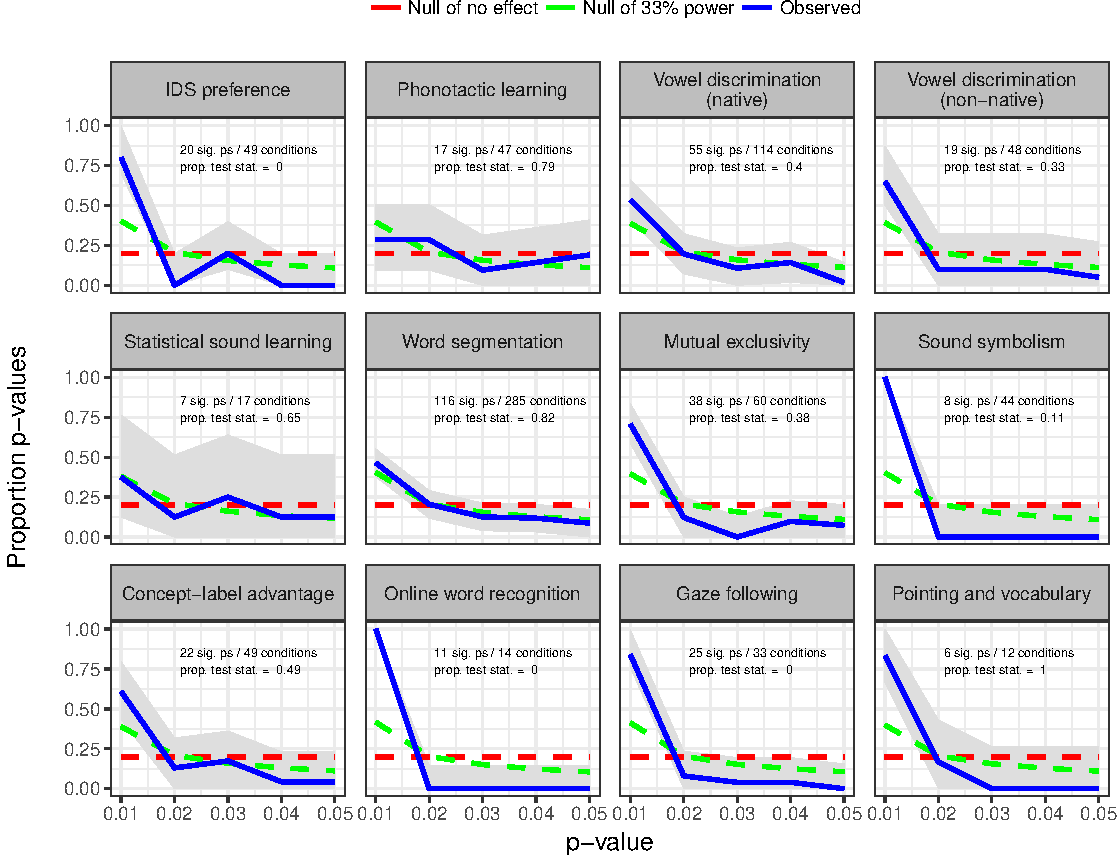
\includegraphics{metalab_synthesis_files/figure-latex/p_curve_plots-1.pdf}
\caption{P-curve for each meta-analysis (Simonsohn, Nelson, \& Simmons,
2014), except those for which p-values were unavailable. In the absense
of p-hacking, we should expect the observed p-curve (blue) to be
right-skewed (more small values). The red dashed line shows the expected
distribution of p-values when the effect is non-existent (the null is
true). The green dashed line shows the expected distribution if the
effect is real, but studies only have 33\% power. {[}WILL FIX LEGEND
LATER{]}}
\end{figure}

A p-curve is the distribution of p-values for the statistical test of
the main hypothesis across a literature (Simonsohn et al., 2014b, 2014a,
2015). Critically, if there is a robust effect in the literature, the
shape of the p-curve should reflect this. In particular, we should
expect the p-curve to be right-skewed with more small values (e.g., .01)
than large values (e.g., .04). An important property of this analysis is
that we should expect this skew independent of any true heterogeneity in
the data, such as age. Evidence that the curve is in fact right-skewed
would suggest that the literature is not biased, and that it provides
evidential value for theory building.

\begin{table}[t]
\footnotesize
\begin{tabular}{lrrrr}
\toprule
\textbf{Phenomenon} & \textbf{\textit{d}} & \textbf{fail-safe-N} & \textbf{funnel skew} & \textbf{p-curve skew}\\
\midrule
IDS preference & 0.71 [0.53, 0.89] & 3762 & 1.88 (0.06) & \\
Phonotactic learning & 0.04 [-0.09, 0.16] & 45 & -1.08 (0.28) & -1.52 (0.06)\\
Vowel discrimination (native) & 0.6 [0.5, 0.71] & 9536 & 8.98 (<.01) & -5.42 (<.01)\\
Vowel discrimination (non-native) & 0.66 [0.42, 0.9] & 3391 & 4.13 (<.01) & -3.24 (<.01)\\
Statistical sound learning & -0.14 [-0.27, -0.02] & Inf & -1.87 (0.06) & \\
Word segmentation & 0.2 [0.15, 0.25] & 5645 & 1.54 (0.12) & -9.67 (<.01)\\
Mutual exclusivity & 1.01 [0.68, 1.33] & 6443 & 6.25 (<.01) & -5 (<.01)\\
Sound symbolism & 0.15 [0.04, 0.26] & 538 & -1.32 (0.19) & -2.16 (0.02)\\
Concept-label advantage & 0.4 [0.29, 0.51] & 3928 & 0.31 (0.76) & -6.15 (0)\\
Online word recognition & 1.89 [0.81, 2.96] & 2843 & 2.92 (<.01) & \\
Gaze following & 0.84 [0.26, 1.42] & 2641 & -1.69 (0.09) & \\
Pointing and vocabulary & 0.41 [0.32, 0.49] & 1202 & 0.59 (0.55) & \\
\bottomrule
\end{tabular}
\caption{Summary of replicability analyses. \textit{d} = Effect size (Cohen's {\it d}) estimated from a random-effect model; fail-safe-N = number of missing studies that would have to exist in order for the overall effect size to be {\it d} = 0; funnel skew = test of asymmetry in funnel plot using the random-effect Egger's test (Stern \& Eggers, 2005); p-curve skew = test of the right skew of the p-curve using the Stouffer method (Simonsohn, Simmons, \& Nelson, 2015); Brackets give 95\% confidence intervals, and parentheses show p-values.}
\end{table}

Figure 2 shows p-curves for 7 of our 12
meta-analyses.\footnote{We did not conduct p-curves on all meta-analyses because previously published meta-analyses did not include the original test statistics in the summary report. In other cases, the key test statistics were inappropriate for p-curve.}
With the exception of phonotactic learning, all p-curves show evidence
of right skew. This is confirmed by formal analyses (Table 2, column 5).

In sum, then, meta-analytic methods, along with our dataset of effect
sizes, provide an opportunity to assess the replicability of the field
of language acquisition. Across a range of analyses, we find that this
literature shows some evidence for bias, but overall, is quite robust.

\section{Theoretical development}\label{theoretical-development}

Next, we turn to how these data can be used to constrain and develop
theories of language acquisition.

Meta-analytic methods provide a precise, quantitative description of the
developmental trajectory of individual phenomena. Figure 3 presents the
developmental trajectories of the phenomena in our dataset at each level
in the linguistic
hierarchy.\footnote{The Pointing and Vocabulary dataset is excluded from this analysis because it does not contain effect sizes at multiple ages.}
By describing how effect sizes change as a function of age, we can begin
to understand what factors might moderate that trajectory, such as
aspects of a child's experience or maturation. For example, the
meta-analysis on mutual-exclusivity (bias for children to select a novel
object, given a novel word; Markman \& Wachtel, 1988) suggests a steep
developmental trajectory of this skill. We can use these data to then
build quantitative models to understand how aspects of experience
(e.g.~vocabulary development) or maturational constraints may be related
to this trajectory (e.g., M. C. Frank, Goodman, \& Tenenbaum, 2009;
McMurray, Horst, \& Samuelson, 2012).

{[}There are also large differences in the relative magnitude of ES of
different skills. Theoretical point about overt skills have larger ES{]}

\begin{figure}[htbp]
\centering
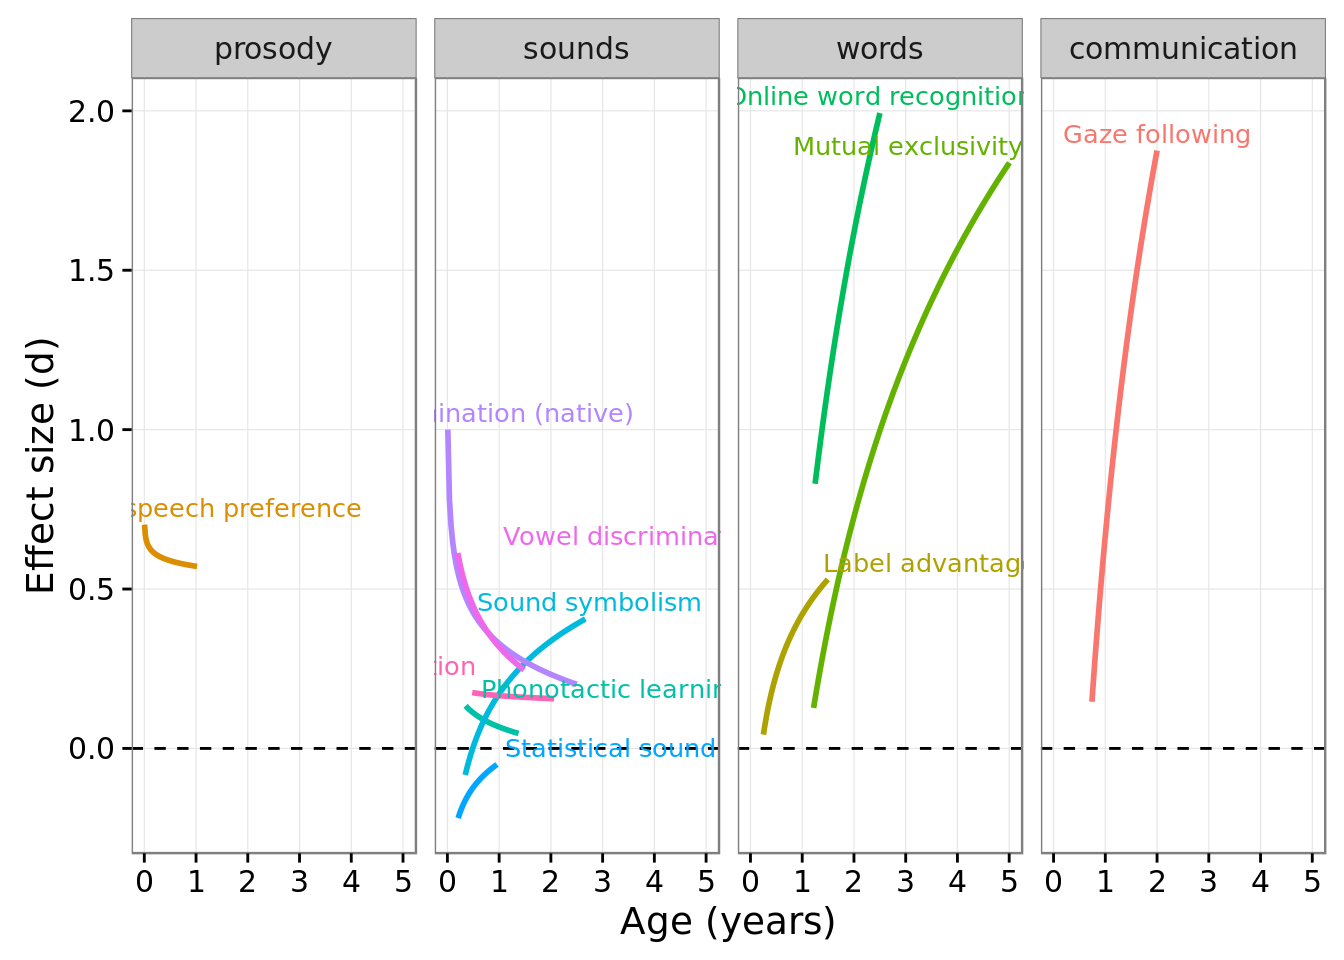
\includegraphics{metalab_synthesis_files/figure-latex/unnamed-chunk-4-1.pdf}
\caption{Effect size plotted as a function of age across all
developmental meta-analyses in our dataset. Lines show logarithmic model
fits. Each point corresponds to a condition, with the size of the point
indicating the number of participants. {[}WILL FIX LABELS LATER{]}}
\end{figure}

\begin{figure}[htbp]
\centering
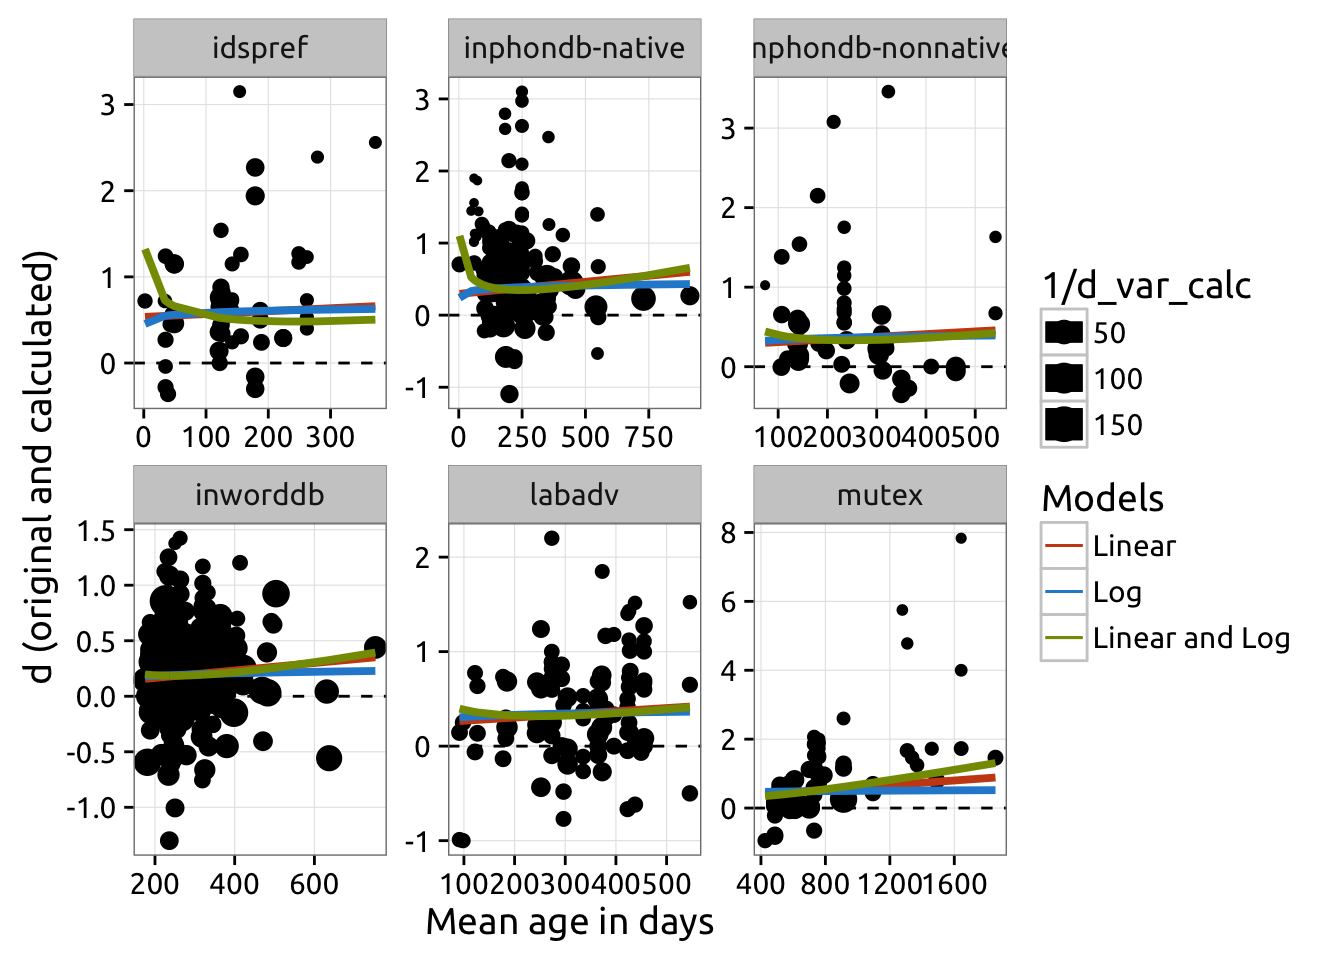
\includegraphics{metalab_synthesis_files/figure-latex/unnamed-chunk-5-1.pdf}
\caption{The left two panels show the developmental trajectories
predicted under different meta-theories of language acqusition. The
bottom-up theory predicts that a child will not begin learning the next
skill in the linguistic hierarchy until the previous skill has been
mastered. The synergistic theory predicts that multiple skills may be
simultaneously acquired. The third panel shows other possible
developmental trajectories for an particular phenomenon (decreasing,
linear, and non-monotonic). The fourth panel shows the observed
meta-analytic data. Effect size is plotted as a function of age from 0-3
years, across 11 different phenomena. These developmental curves suggest
there is interactivity across language skills, rather than bottom-up,
sequential learning of the linguistic hierarchy.}
\end{figure}

In addition, meta-analytic methods provide an approach for synthesizing
across different linguistic skills via the language of effect sizes. The
ultimate goal is to use meta-analytic data to build a single,
quantitative model of the language acquisition system, much like those
developed for individual language acquisition phenomena, like word
learning. Developing a single quantitative model is a lofty goal,
however, and will likely require much more precise description of the
phenomena than is available in our dataset. Nevertheless, we can use our
data to distinguish between broad meta-theories about the relationship
between different skills.

There are two existing meta-theories in the literature about the
dependencies between different skills in language acquisition. The
first---the \enquote{bottom-up} theory---proposes that linguistic skills
are acquired sequentially beginning with skills at the lowest level of
the linguistic hierarchy. Under this theory, once a skill is mastered,
it can be used to support the acquisition of skills higher in the
linguistic hierarchy. In this way, a child sequentially acquires the
skills of language, \enquote{bootstrapping} from existing knowledge at
lower levels to new knowledge at higher levels. There is a wide range of
evidence consistent with this view. For example, there is evidence that
prosody supports the acquisition of sound categories {[}CITE{]}, word
boundaries {[}CITE{]}, and even word learning (e.g., Shukla, White, \&
Aslin, 2011).

A second possibility is that there is interactivity in the language
system such that multiple skills are learned simultaneously across the
system. Under this proposal, a child does not wait to begin learning the
meanings of words until the sounds of a language are mastered, for
example; rather, the child is jointly solving the problem of word
learning in concert other language skills. This possibility is
consistent with predictions of a class of hierarchical Bayesian models
that suggest that more abstract knowledge may be acquired quickly,
before lower level information, and may in turn support the acquisition
of lower information (``blessing of abstraction,'' Goodman, Ullman, \&
Tenenbaum, 2011). There is evidence for this proposal from work that
suggests word learning supports the acquisition of lower-level
information like phonemes (Feldman, Myers, White, Griffiths, \& Morgan,
2013). More broadly, there is evidence that higher level skills like
word learning may be acquired relatively early in development, likely
before lower level skills have been mastered (e.g., Bergelson \&
Swingley, 2012).

Within the meta-analytic framework, we can represent these two theories
schematically by plotting the effect sizes for different skills across
development. Figure 4 (left) shows the predicted pattern by the
bottom-up theory (left) and the interactive theory (left center). We can
also specifiy an infinite number of other possible trajectories by
varying the functional form and parameters of the model. Figure 4 (right
center; \enquote{ad hoc}) shows several other possible trajectories. For
example, we might expect that a skill might have a non-monotonic
trajectory, increasing with age, and then decreasing. By specifying the
shape of these developmental trajectorries and the age at which
acquisition begins, we can consider many possible theories and
meta-theories of development.

Our data allow us to begin to differentiate between this space of
theories. Figure 4 (right) presents a synthetic representation of the
developmental trajectories of all the skills in our dataset. We find
strong evidence for interactivity---children begin learning even
high-level skills, like the meanings of words, early in development, and
even low-level skills like sound categories show a protracted period of
development. Moving forward, we can use this approach to distinguish
between a larger space of meta-theories and, ultimately, build a single
quantitative theory of language acquisition.

\section{Discussion}\label{discussion}

Building a theory of a complex psychological phenomenon requires making
good inductive inferences from the available data. We suggest that
meta-analysis can support this process by allowing the researcher to
verdically describe the to-be-explained behavior, and to do so with
high-fidelity. Here, we apply the meta-analytic toolkit to the domain of
language acquisition---a domain where there are concerns of
replicability, and where high-fidelity data is needed to explain its
complexity. We find that the existing literature in this domain describe
robust phenomena and thus should form the basis of theory development.
We then offer a preliminary synthesis of the field by aggregating across
language acquisition phenomena. We find evidence that linguistic skills
are acquired interactively rather than in a strictly bottom-up fashion.

There are a number of important limitations to the meta-analytic
approach as a theoretical tool. First, this method relies on researchers
conducting replications of the same study across a range of ages and,
critically, reporting these data so that they can be used in
meta-analyses. To the extent that researchers do not conduct these
studies, or report the necessary statistics in their write-ups (e.g.,
means and standard deviations), the meta-analytic method cannot be
applied. Second, the meta-analytic method, as in the case of
qualitiative forms of synthesis (e.g.~literature review), is limited by
the potential presence of bias, which can come from a ranges of sources
including non-representative participant populations, failure to publish
null findings, and analytical degrees-of-freedom. To the extent these
biases are present in the literature, methods of synthesizing these
findings will also be biased.

In addition, there are a number of more substantive concerns with this
method. One possibility is that the magnitude of effect may be more
related to the method than the psychological phenomenon. While this may
be true to some extent, we find that method does not have a large impact
on effect size for a phenomena, relative to other moderators like age
(see SI). Another issue is that meta-analysis usually measures signal to
noise, not units of interest (e.g.~ability in an absolute sense), so
there could be important confounds with respect to this.

SHO {[}Issue of heterogenity{]}: I am still not quite sure which would
be my ideal solution - but if we leave the MAs in as is, at least those
limitations should go in the discussion? Could be an interesting point
about how our MAs might be in an uncanny valley region where we have
enough data to aggregate, but still have potentially very noisy measure
if we do not take care what exactly we aggregate (take native vowels -
if we had 100 more measures maybe also that noisy set would show a
positive development?!)

SHO: It feels like the paper is building up the \enquote{Theoretical
Development} section; first we validate that the effects in the
meta-analyses are real, and then we build an overarching model. When I
got to that section though I didn't fully understand what I was looking
at. I had questions like, why log over linear curves? Just because it's
a better fit of the data? What does that say about development? You
comment that levels seem to be overlapping. Is that true for all levels
or do lower levels overlap more than higher levels overlap? I think this
section could benefit from more explanation of what we're seeing in the
figures as it specifically relates to development. At the same time, I
think a more detailed explanation of what is needed / to come to get a
clearer picture of what is happening in development would be great. For
example, do we need more meta-analyses within a specific level, more age
groups, etc.?

Future directions:

\begin{itemize}
\item
  Educational tool - presage/link to other paper
\item
  Contributions, CAMAS
\item
  Other domains -- language acquisition as a case study
\end{itemize}

TO DO:

\begin{itemize}
\item
  discussion
\item
  figure out what's going on with statistical sound learning.
\item
  figure out what's going on with vowel discrimination (native)
\item
  model fits on the meta-meta
\item
  abstract
\item
  reliability analyses
\item
  clean up figures
\end{itemize}

\paragraph{Author Contributions}\label{author-contributions}

\paragraph{Acknowledgments}\label{acknowledgments}

\newpage

\subsubsection{References}\label{references}

\setlength{\parindent}{-0.5in} \setlength{\leftskip}{0.5in}
\setlength{\parskip}{8pt}

\hypertarget{refs}{}
\hypertarget{ref-anderson2016response}{}
Anderson, C. J., Bahník, Š., Barnett-Cowan, M., Bosco, F. A., Chandler,
J., Chartier, C. R., \ldots{} others. (2016). Response to comment on
``estimating the reproducibility of psychological science''.
\emph{Science}, \emph{351}(6277), 1037--1037.

\hypertarget{ref-bergelson2016}{}
Bergelson, E., \& Swingley, D. (2012). At 6--9 months, human infants
know the meanings of many common nouns. \emph{Proceedings of the
National Academy of Sciences}, \emph{109}(9), 3253--3258.

\hypertarget{ref-bergmann2015development}{}
Bergmann, C., \& Cristia, A. (2015). Development of infants'
segmentation of words from native speech: A meta-analytic approach.
\emph{Developmental Science}.

\hypertarget{ref-button2013power}{}
Button, K. S., Ioannidis, J. P., Mokrysz, C., Nosek, B. A., Flint, J.,
Robinson, E. S., \& Munafò, M. R. (2013). Power failure: Why small
sample size undermines the reliability of neuroscience. \emph{Nature
Reviews Neuroscience}, \emph{14}(5), 365--376.

\hypertarget{ref-dunst2012preference}{}
Dunst, C., Gorman, E., \& Hamby, D. (2012). Preference for
infant-directed speech in preverbal young children. \emph{Center for
Early Literacy Learning}, \emph{5}(1).

\hypertarget{ref-feldman2013word}{}
Feldman, N. H., Myers, E. B., White, K. S., Griffiths, T. L., \& Morgan,
J. L. (2013). Word-level information influences phonetic learning in
adults and infants. \emph{Cognition}, \emph{127}(3), 427--438.

\hypertarget{ref-frank2009using}{}
Frank, M. C., Goodman, N. D., \& Tenenbaum, J. B. (2009). Using
speakers' referential intentions to model early cross-situational word
learning. \emph{Psychological Science}, \emph{20}(5), 578--585.

\hypertarget{ref-frank2016performance}{}
Frank, M. C., Lewis, M. L., \& MacDonald, K. (in press). A performance
model for early word learning. In \emph{Proceedings of the 38th Annual
Conference of the Cognitive Science Society}. Retrieved from
\url{http://langcog.stanford.edu/papers_new/frank-2016-underrev.pdf}

\hypertarget{ref-Gilbert1037}{}
Gilbert, D. T., King, G., Pettigrew, S., \& Wilson, T. D. (2016).
Comment on Estimating the reproducibility of psychological science.
\emph{Science}, \emph{351}(6277), 1037--1037.
doi:\href{https://doi.org/10.1126/science.aad7243}{10.1126/science.aad7243}

\hypertarget{ref-goodman2011learning}{}
Goodman, N. D., Ullman, T. D., \& Tenenbaum, J. B. (2011). Learning a
theory of causality. \emph{Psychological Review}, \emph{118}(1), 110.

\hypertarget{ref-ioannidis2005most}{}
Ioannidis, J. P. (2005). Why most published research findings are false.
\emph{PLoS Med}, \emph{2}(8), e124.

\hypertarget{ref-lfprep}{}
Lewis, M., \& Frank, M. C. (in prep). Multiple routes to disambiguation.

\hypertarget{ref-markman1988}{}
Markman, E., \& Wachtel, G. (1988). Children's use of mutual exclusivity
to constrain the meanings of words. \emph{Cognitive Psychology},
\emph{20}(2), 121--157.

\hypertarget{ref-mcmurray2012word}{}
McMurray, B., Horst, J. S., \& Samuelson, L. K. (2012). Word learning
emerges from the interaction of online referent selection and slow
associative learning. \emph{Psychological Review}, \emph{119}(4), 831.

\hypertarget{ref-open2012open}{}
Open Science Collaboration. (2012). An open, large-scale, collaborative
effort to estimate the reproducibility of psychological science.
\emph{Perspectives on Psychological Science}, \emph{7}(6), 657--660.

\hypertarget{ref-open2015estimating}{}
Open Science Collaboration. (2015). Estimating the reproducibility of
psychological science. \emph{Science}, \emph{349}(6251), aac4716.

\hypertarget{ref-orwin1983fail}{}
Orwin, R. G. (1983). A fail-safe n for effect size in meta-analysis.
\emph{Journal of Educational Statistics}, 157--159.

\hypertarget{ref-Peterson:2016}{}
Peterson, D. (2016). The Baby Factory: Difficult Research Objects,
Disciplinary Standards, and the Production of Statistical Significance.
\emph{Socius: Sociological Research for a Dynamic World}, \emph{2}(0),
1--10.

\hypertarget{ref-shukla2011prosody}{}
Shukla, M., White, K. S., \& Aslin, R. N. (2011). Prosody guides the
rapid mapping of auditory word forms onto visual objects in 6-mo-old
infants. \emph{Proceedings of the National Academy of Sciences},
\emph{108}(15), 6038--6043.

\hypertarget{ref-simonsohn2014power}{}
Simonsohn, Nelson, L. D., \& Simmons, J. P. (2014a). P-curve and effect
size correcting for publication bias using only significant results.
\emph{Perspectives on Psychological Science}, \emph{9}(6), 666--681.

\hypertarget{ref-simonsohn2014p}{}
Simonsohn, Nelson, L. D., \& Simmons, J. P. (2014b). P-curve: A key to
the file-drawer. \emph{Journal of Experimental Psychology: General},
\emph{143}(2), 534.

\hypertarget{ref-simonsohn2015better}{}
Simonsohn, Simmons, J. P., \& Nelson, L. D. (2015). Better p-curves.
\emph{Simonsohn, Uri, Joseph P. Simmons, and Leif D. Nelson
(Forthcoming),``Better P-Curves,'' Journal of Experimental Psychology:
General}.

\hypertarget{ref-sterne2005regression}{}
Sterne, J. A., \& Egger, M. (2005). Regression methods to detect
publication and other bias in meta-analysis. \emph{Publication Bias in
Meta-Analysis: Prevention, Assessment, and Adjustments}, 99--110.

\hypertarget{ref-tsuji2014perceptual}{}
Tsuji, S., \& Cristia, A. (2014). Perceptual attunement in vowels: A
meta-analysis. \emph{Developmental Psychobiology}, \emph{56}(2),
179--191.



\end{document}
